\section{Règles d'associations}

Pour cette section, le filtre \textit{NumericToNominal} a été appliqué aux attributs \textit{NumberCarsOwned}, \textit{YearlyIncome} et \textit{TotalChildren}.

Seul les algorithmes \textit{Apriori} et \textit{FilteredAssociator} ont été testé. Seul ceux-ci étaient disponible (voir \ref{associate}).

\begin{figure}[H]
    \centering
    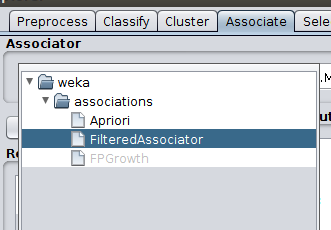
\includegraphics[width=0.5\linewidth, fbox]{img/associate.png}
    \caption{Règles d'associations : Algos disponible}
    \label{associate}
\end{figure}

\subsection{Apriori}

Le seuil minimum de confiance a été modifié pour obtenir plus de règles.

Voici les paramètres :

\begin{lstlisting}
Apriori -N 10 -T 0 -C 0.8 -D 0.05 -U 1.0 -M 0.1 -S -1.0 -c 1
\end{lstlisting}

Et le résultat (figure \ref{apriori}).

\begin{figure}[H]
    \centering
	\makebox[\textwidth][c]{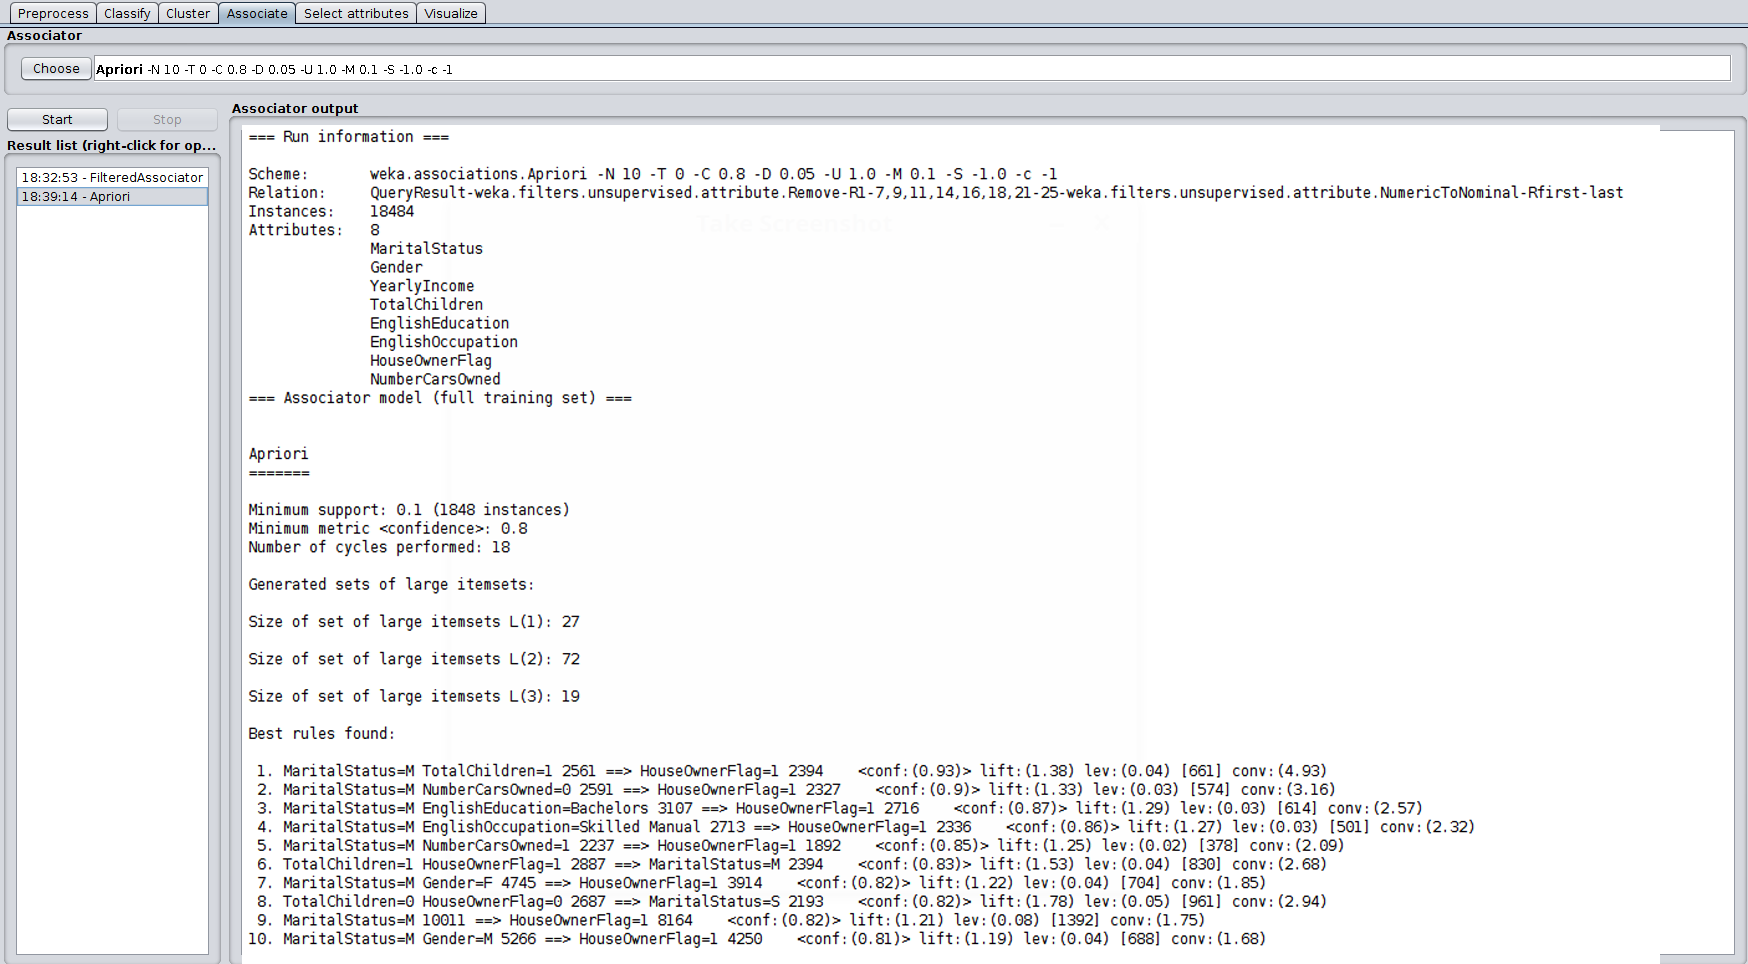
\includegraphics[width=1.3\linewidth, fbox]{img/apriori.png}}%
    \caption{Règles d'associations : Apriori résultat}
    \label{apriori}
\end{figure}

\subsection{FilteredAssociator}

Cet algorithme permet de créer des règles d'association filtrées.

Les 10 règles obtenues (figure \ref{filtered}) sont identiques au résultat de l'\textit{Apriori}.

\begin{figure}[H]
    \centering
	\makebox[\textwidth][c]{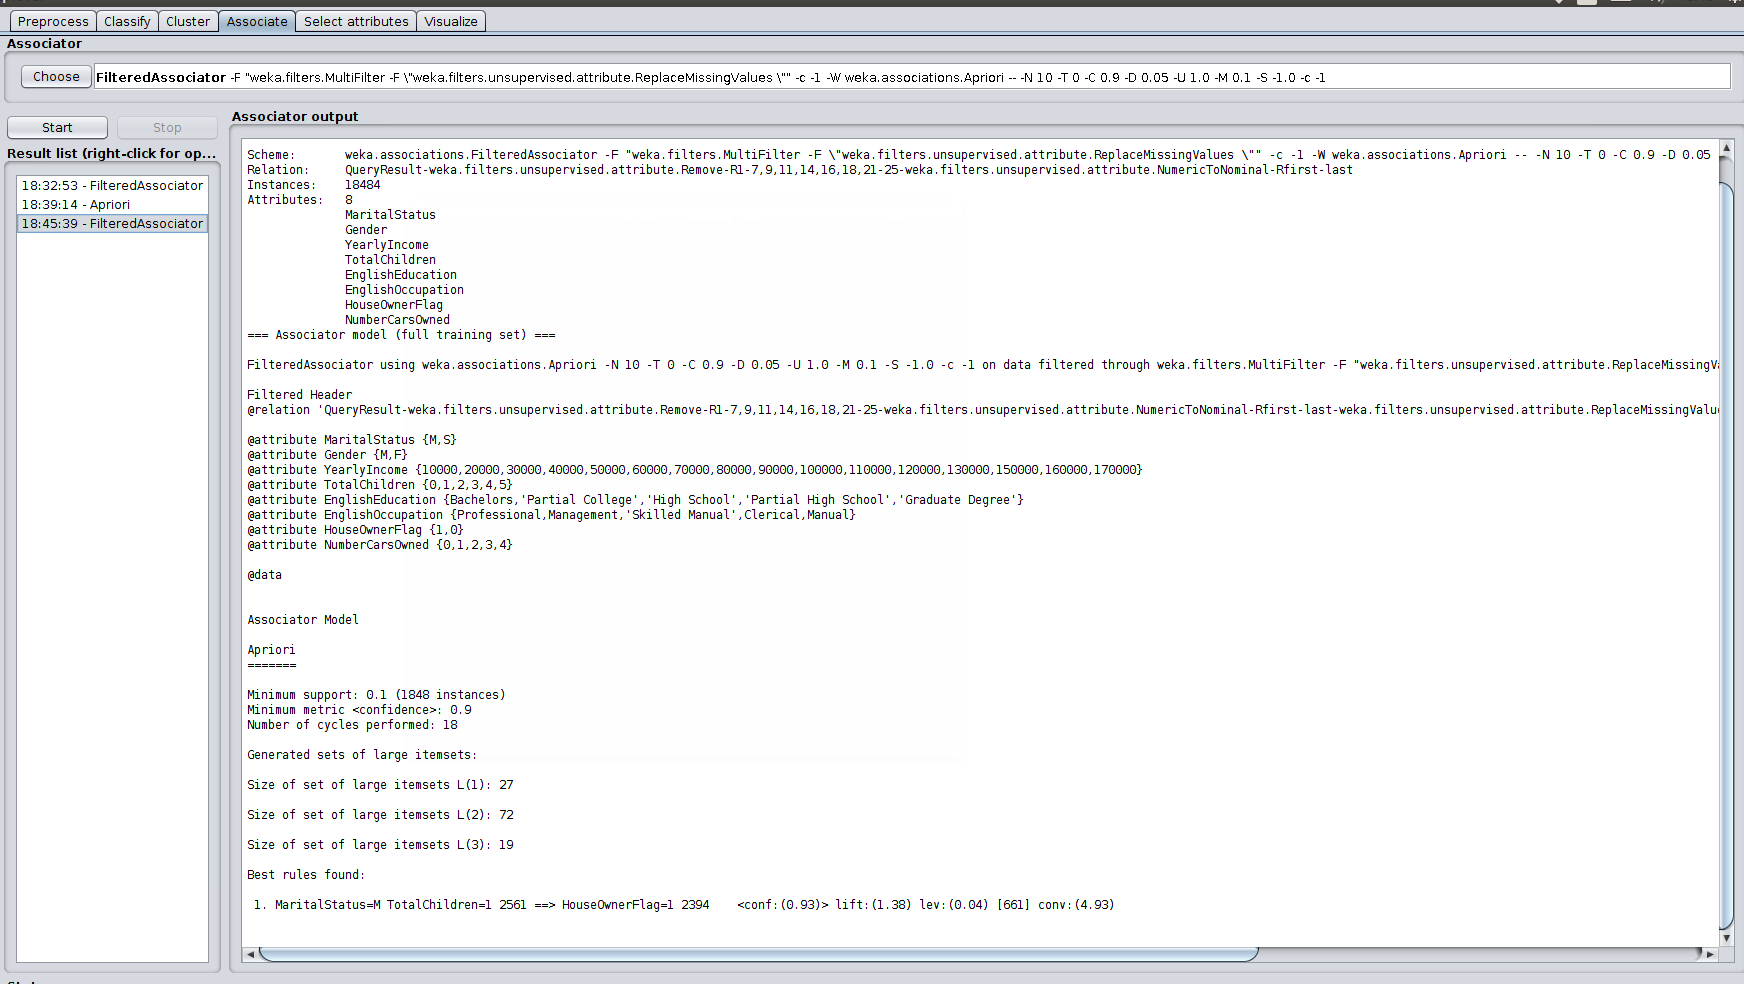
\includegraphics[width=1.3\linewidth, fbox]{img/filtered.png}}%
    \caption{Règles d'associations : FilteredAssociator résultat}
    \label{filtered}
\end{figure}
